% !TeX program = xelatex
\documentclass{article}
\usepackage{xeCJK}
\usepackage{tikz}
\usepackage[outline]{contour}
\usepackage{graphicx}
\graphicspath{ {./} }
\setCJKmainfont{Kaiti SC}
% \setCJKmainfont{Xingkai SC}
% \setCJKmainfont{STKaiti}

\newcommand\Grid[1]{%
 \tikz[baseline=(char.base)]{%
  \draw[xstep=1ex,ystep=1ex,help lines] (-1ex,-1ex) grid (1ex,1ex);
  \draw[help lines,densely dash dot]
  (-1ex,-1ex) -- (1ex,1ex)  (-1ex,1ex) -- (1ex,-1ex);
  \node[inner sep=0pt] (char) at (0,0) {#1};
 }%
}
\pagenumbering{gobble}
\begin{document}
\begin{center}
    \Huge 江南 \\
\end{center}
\begin{flushright}
    \huge 汉 $\bullet$ 汉乐府 \\
\end{flushright}
\begin{center}
    \Huge 江南可采莲 \\
    \Huge 莲叶何田田 \\
    \Huge 鱼戏荷叶间 \\
    \Huge 鱼戏荷叶东 \\
    \Huge 鱼戏荷叶西 \\
    \Huge 鱼戏荷叶南 \\
    \Huge 鱼戏荷叶北 \\
\end{center}
\hrule
\begin{center}
    \Huge \Grid{江}\Grid{南}\Grid{可}\Grid{采}\Grid{莲} \\
\end{center}
\begin{flushright}
    \huge \Grid{汉} $\bullet$ \Grid{汉}\Grid{乐}\Grid{府} \\
\end{flushright}
\begin{center}
    \Huge \Grid{江}\Grid{南}\Grid{可}\Grid{采}\Grid{莲} \\
    \Huge \Grid{莲}\Grid{叶}\Grid{何}\Grid{田}\Grid{田} \\
    \Huge \Grid{鱼}\Grid{戏}\Grid{荷}\Grid{叶}\Grid{间} \\
    \Huge \Grid{鱼}\Grid{戏}\Grid{荷}\Grid{叶}\Grid{东} \\
    \Huge \Grid{鱼}\Grid{戏}\Grid{荷}\Grid{叶}\Grid{西} \\
    \Huge \Grid{鱼}\Grid{戏}\Grid{荷}\Grid{叶}\Grid{南} \\
    \Huge \Grid{鱼}\Grid{戏}\Grid{荷}\Grid{叶}\Grid{北} \\
\end{center}
\hrule
\newpage
\begin{figure}
    \centering
    \makebox[0pt]{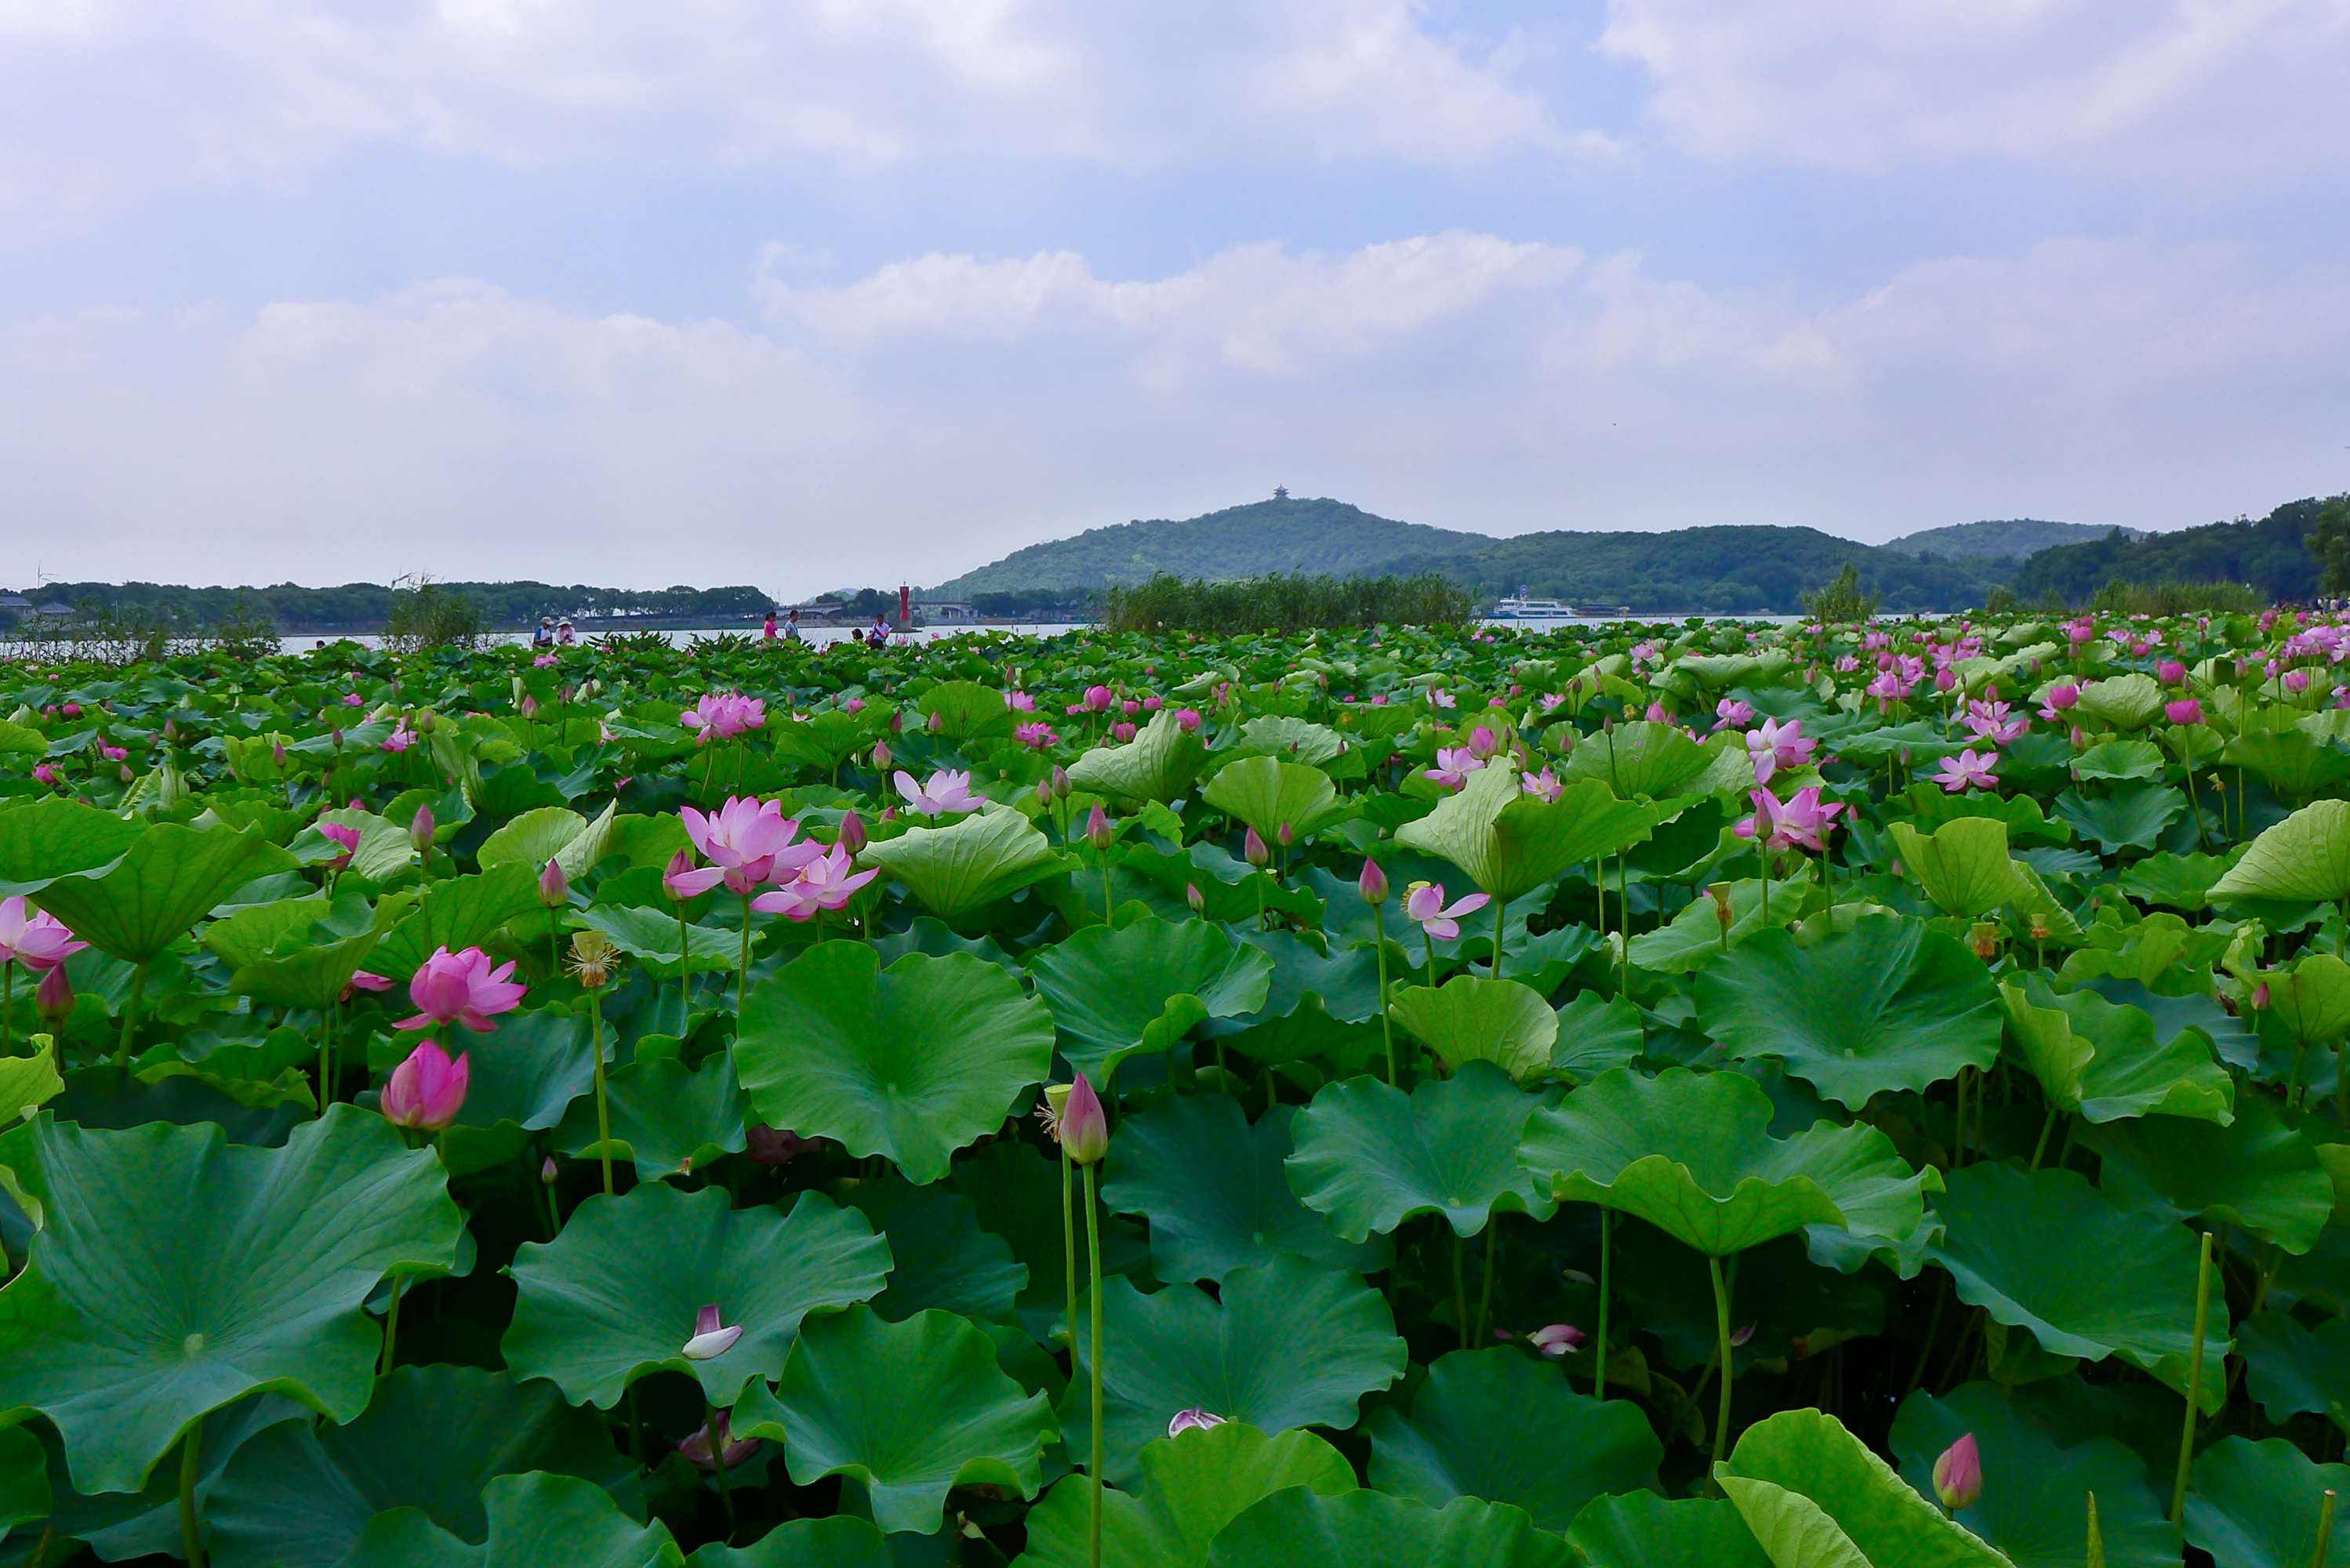
\includegraphics[width=0.9\paperwidth]{FTwCq73agAA8_jy.jpeg}}
\end{figure}
\begin{figure}
    \centering
    \makebox[0pt]{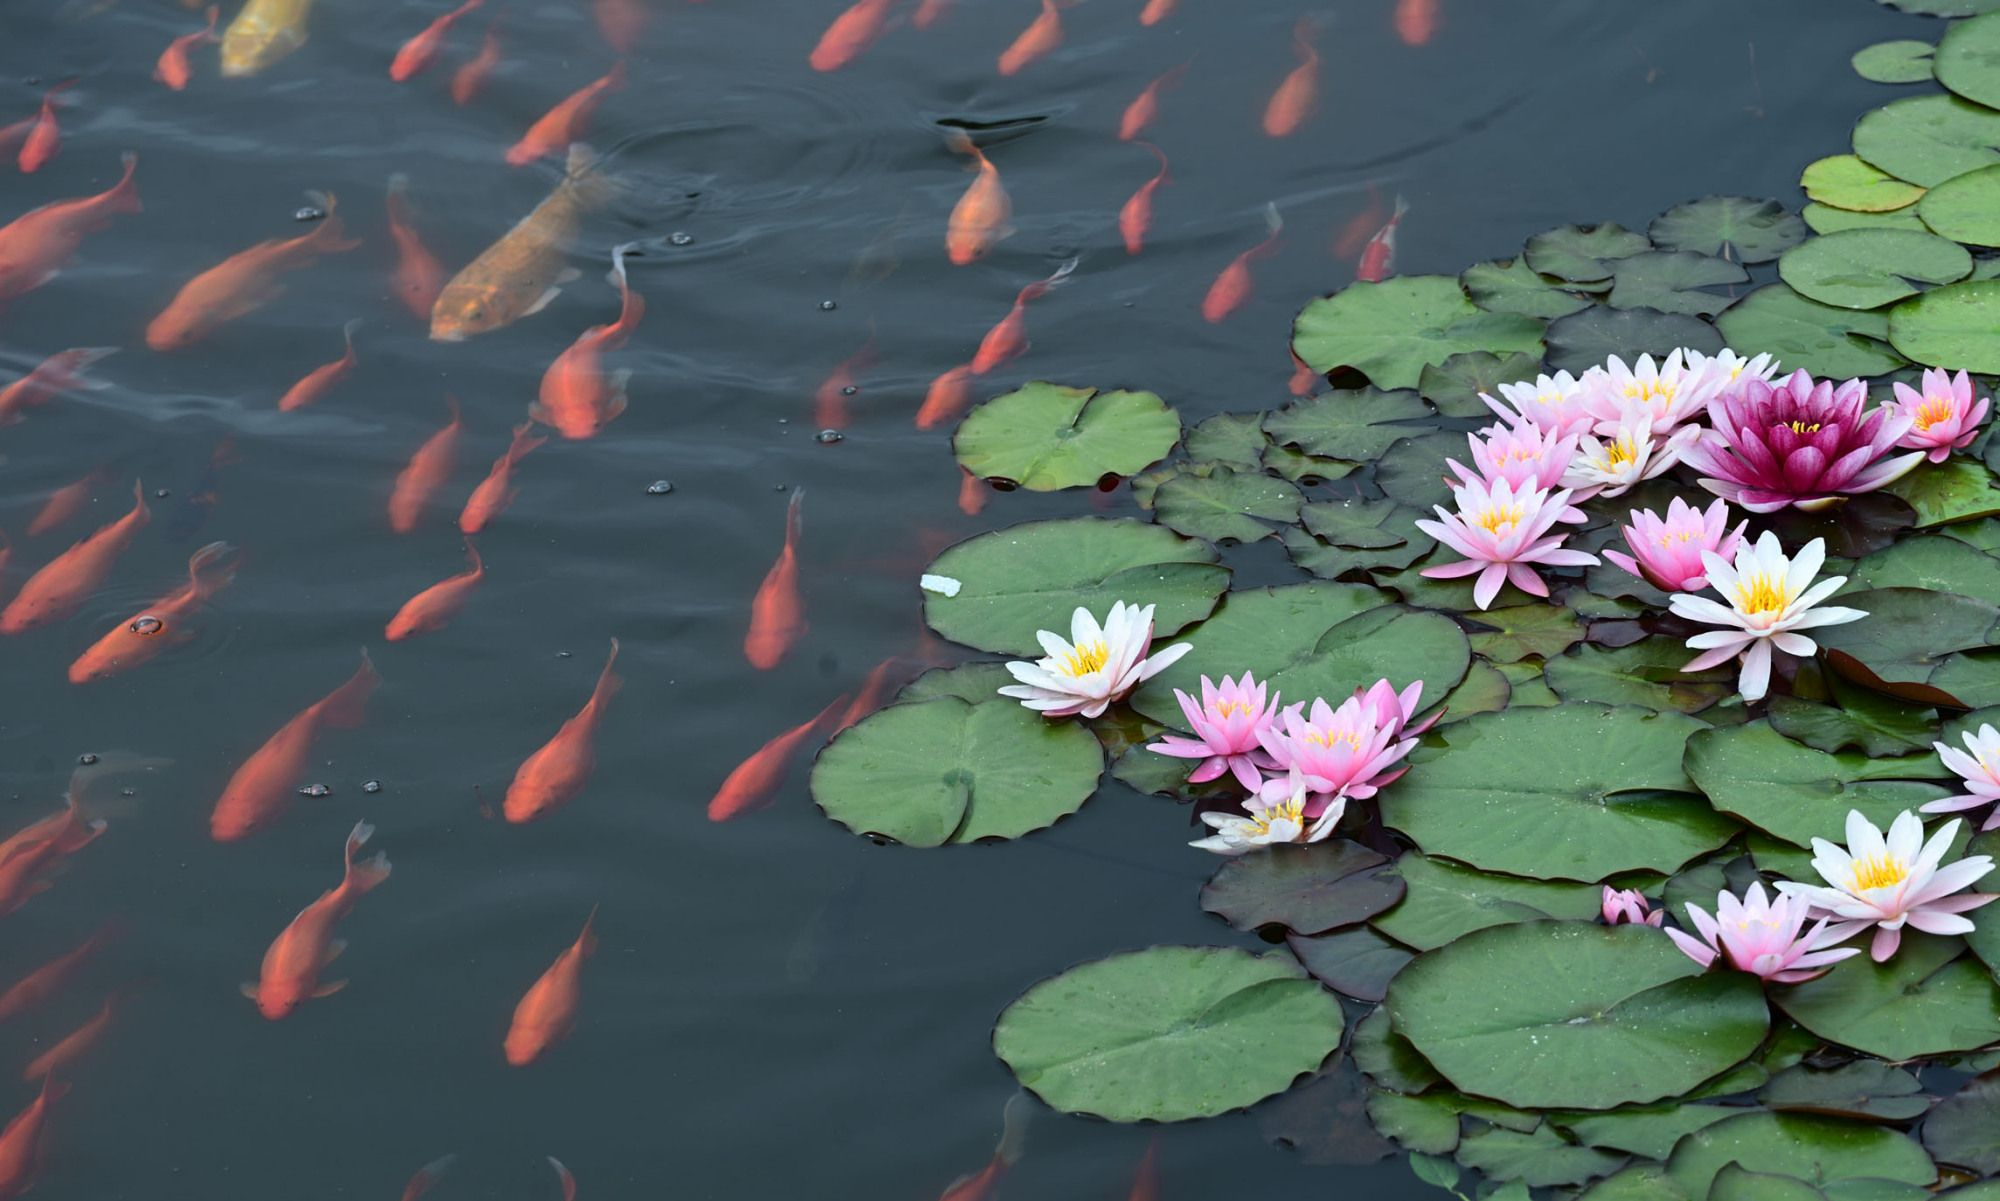
\includegraphics[width=0.9\paperwidth]{a8c9-iurnkpq8031874.jpg}}
\end{figure}
\begin{figure}
    \centering
    \makebox[0pt]{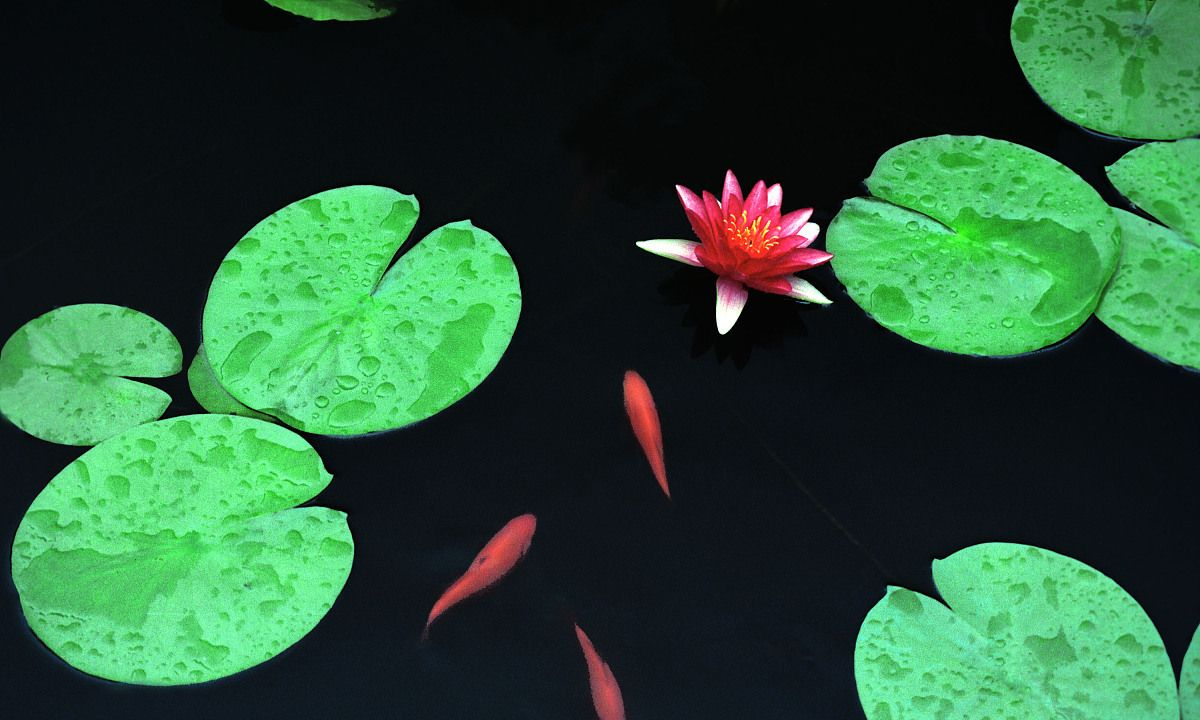
\includegraphics[width=0.9\paperwidth]{022f-iurnkpq8032972.jpg}}
\end{figure}
\end{document}